\section{Auswertung}
\label{sec:Auswertung}

\subsection{Bragg-Bedingung}
\label{sec:Bragg}

Die Messwerte zur Überprüfung der Bragg-Bedingung sind in \autoref{tab:Bragg} zu finden und in \autoref{fig:bragg}
dargestellt. Es wurde ein Maxium bei $27,7^{\circ}$ festgestellt. Nachdem Reflexionsgesetz liegt der
theoretische Winkel bei $28^{\circ}$. Daraus ergibt sich eine Abweichung von $1,5\%$.

\begin{table}
  \centering
  \begin{tabular}{c c | c c}
    \toprule
    $\theta^{\circ}$ & $N/Imp/s$ & $\theta^{\circ}$ & $N/Imp/s$ \\
    \midrule
    26,0 &  39,0 & 28,2 & 272,0 \\
    26,1 &  43,0 & 28,3 & 263,0 \\
    26,2 &  43,0 & 28,4 & 255,0 \\
    26,3 &  52,0 & 28,5 & 247,0 \\
    26,4 &  76,0 & 28,6 & 234,0 \\
    26,5 &  85,0 & 28,7 & 236,0 \\
    26,6 & 113,0 & 28,8 & 222,0 \\
    26,7 & 117,0 & 28,9 & 206,0 \\
    26,8 & 146,0 & 29,0 & 181,0 \\
    26,9 & 164,0 & 29,1 & 185,0 \\
    27,0 & 183,0 & 29,2 & 164,0 \\
    27,1 & 182,0 & 29,3 & 155,0 \\
    27,2 & 216,0 & 29,4 & 154,0 \\
    27,3 & 219,0 & 29,5 & 129,0 \\
    27,4 & 238,0 & 29,6 & 110,0 \\
    27,5 & 256,0 & 29,7 & 100,0 \\
    27,6 & 281,0 & 29,8 &  90,0 \\
    27,7 & 277,0 & 29,9 &  84,0 \\
    27,8 & 274,0 & 30,0 &  75,0 \\
    27,9 & 269,0 & & \\
    28,0 & 278,0 & & \\
    28,1 & 274,0 & & \\
    \bottomrule
  \end{tabular}
  \caption{Messwerte zur Überrüfung der Bragg-Bedingung.}
  \label{tab:Bragg}
\end{table}

\begin{figure}
  \centering
  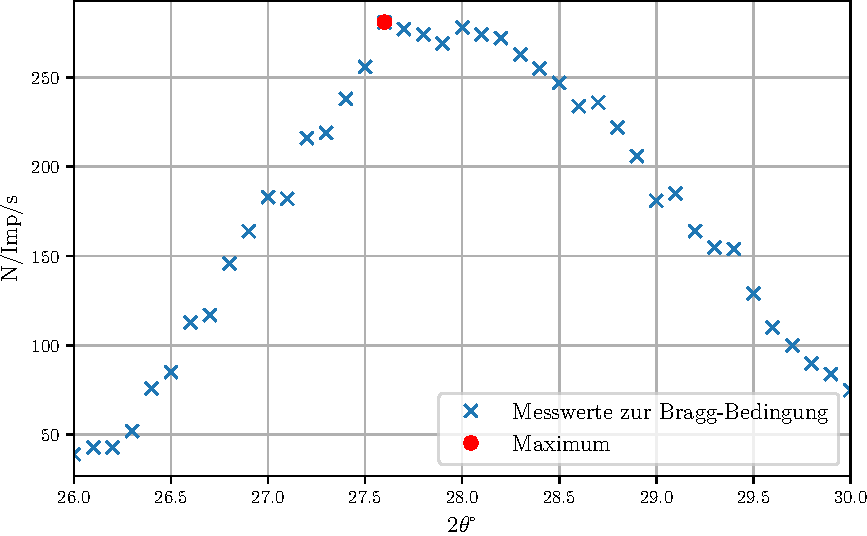
\includegraphics{bragg.pdf}
  \caption{Werte zur Bestimmung der Bragg-Bedingung.}
  \label{fig:bragg}
\end{figure}

\subsection{Emissionsspektrum der Cu-Röntgenröhre}
\label{sec:cu}
Die Messwerte des Emissionsspektrums der Kupferröntgenröhre sind in \autoref{tab:Cu} dargestellt. Weiterhin sind Die
Messwerte des Detailspektrums in \autoref{tab:Detailspektrum} zu finden.

\begin{table}
  \centering
  \begin{tabular}{c c | c c | c c}
    \toprule
    $\theta^{\circ}$ & $N/Imp/s$ & $\theta^{\circ}$ & $N/Imp/s$ & $\theta^{\circ}$ & $N/Imp/s$ \\
    \midrule
     4,0 &  40,0 & 11,2 & 409,0 & 18,6 &  176,0 \\
     4,2 &  42,0 & 11,4 & 411,0 & 18,8 &  158,0 \\
     4,4 &  38,0 & 11,6 & 403,0 & 19,0 &  161,0 \\
     4,6 &  34,0 & 11,8 & 393,0 & 19,2 &  154,0 \\
     4,8 &  37,0 & 12,0 & 381,0 & 19,4 &  152,0 \\
     5,0 &  60,0 & 12,2 & 385,0 & 19,6 &  150,0 \\
     5,2 &  70,0 & 12,4 & 389,0 & 19,8 &  200,0 \\
     5,4 & 113,0 & 12,6 & 389,0 & 20,0 & 1374,0 \\
     5,6 & 130,0 & 12,8 & 374,0 & 20,2 & 1437,0 \\
     5,8 & 144,0 & 13,0 & 370,0 & 20,4 & 1021,0 \\
     6,0 & 167,0 & 13,2 & 351,0 & 20,6 &  230,0 \\
     6,2 & 189,0 & 13,4 & 322,0 & 20,8 &  205,0 \\
     6,4 & 201,0 & 13,6 & 294,0 & 21,0 &  185,0 \\
     6,6 & 221,0 & 13,8 & 277,0 & 21,2 &  177,0 \\
     6,8 & 238,0 & 14,0 & 273,0 & 21,4 &  169,0 \\
     7,0 & 273,0 & 14,2 & 270,0 & 21,6 &  179,0 \\
     7,2 & 279,0 & 14,4 & 263,0 & 21,8 &  194,0 \\
     7,4 & 299,0 & 14,6 & 261,0 & 22,0 &  269,0 \\
     7,6 & 296,0 & 14,8 & 244,0 & 22,2 & 2417,0 \\
     7,8 & 304,0 & 15,0 & 250,0 & 22,4 & 4662,0 \\
     8,0 & 329,0 & 15,2 & 247,0 & 22,6 & 4345,0 \\
     8,2 & 335,0 & 15,4 & 244,0 & 22,8 & 1292,0 \\
     8,4 & 333,0 & 15,6 & 237,0 & 23,0 &  182,0 \\
     8,6 & 351,0 & 15,8 & 244,0 & 23,2 &  142,0 \\
     8,8 & 366,0 & 16,0 & 224,0 & 23,4 &  124,0 \\
     9,0 & 377,0 & 16,2 & 221,0 & 23,6 &  114,0 \\
     9,2 & 375,0 & 16,4 & 224,0 & 23,8 &  109,0 \\
     9,4 & 385,0 & 16,6 & 218,0 & 24,0 &  104,0 \\
     9,6 & 376,0 & 16,8 & 203,0 & 24,2 &  103,0 \\
     9,8 & 395,0 & 17,0 & 197,0 & 24,4 &   91,0 \\
    10,0 & 414,0 & 17,2 & 200,0 & 24,6 &   87,0 \\
    10,2 & 416,0 & 17,4 & 196,0 & 24,8 &   91,0 \\
    10,4 & 408,0 & 17,6 & 188,0 & 25,0 &   84,0 \\
    10,6 & 417,0 & 17,8 & 186,0 & 25,2 &   81,0 \\
    10,8 & 403,0 & 18,0 & 170,0 & 25,4 &   77,0 \\
    11,0 & 424,0 & 18,2 & 174,0 & 25,6 &   78,0 \\
    11,2 & 409,0 & 18,4 & 165,0 & 25,8 &   76,0 \\
         &       &      &       & 26,0 &   79,0 \\
    \bottomrule
  \end{tabular}
  \caption{Messwerte der Kupferröntgenröhre.}
  \label{tab:Cu}
\end{table}

\begin{table}
  \centering
  \begin{tabular}{c c | c c}
    \toprule
    $\theta^{\circ}$ & $N/Imp/s$ & $\theta^{\circ}$ & $N/Imp/s$ \\
    \midrule
    19,0 &  158,0 & 21.4 &  170,0 \\
    19,1 &  154,0 & 21.5 &  175,0 \\
    19,2 &  164,0 & 21.6 &  182,0 \\
    19,3 &  149,0 & 21.7 &  198,0 \\
    19,4 &  151,0 & 21.8 &  187,0 \\
    19,5 &  145,0 & 21.9 &  218,0 \\
    19,6 &  157,0 & 22.0 &  263,0 \\
    19,7 &  173,0 & 22.1 &  590,0 \\
    19,8 &  200,0 & 22.2 & 2305,0 \\
    19,9 &  688,0 & 22.3 & 4041,0 \\
    20,0 & 1392,0 & 22.4 & 4691,0 \\
    20,1 & 1473,0 & 22.5 & 4443,0 \\
    20,2 & 1439,0 & 22.6 & 4386,0 \\
    20,3 & 1413,0 & 22.7 & 3122,0 \\
    20,4 & 1040,0 & 22.8 & 1407,0 \\
    20,5 &  391,0 & 22.9 &  232,0 \\
    20,6 &  237,0 & 23.0 &  167,0 \\
    20,7 &  212,0 & 23.1 &  150,0 \\
    20,8 &  197,0 & 23.2 &  142,0 \\
    20,9 &  191,0 & 23.3 &  132,0 \\
    21,0 &  181,0 & 23.4 &  128,0 \\
    21,1 &  176,0 & & \\
    21,2 &  178,0 & & \\
    21,3 &  175,0 & & \\
    \bottomrule
  \end{tabular}
  \caption{Messwerte des Detailspektrums.}
  \label{tab:Detailspektrum}
\end{table}

\begin{figure}
  \centering
  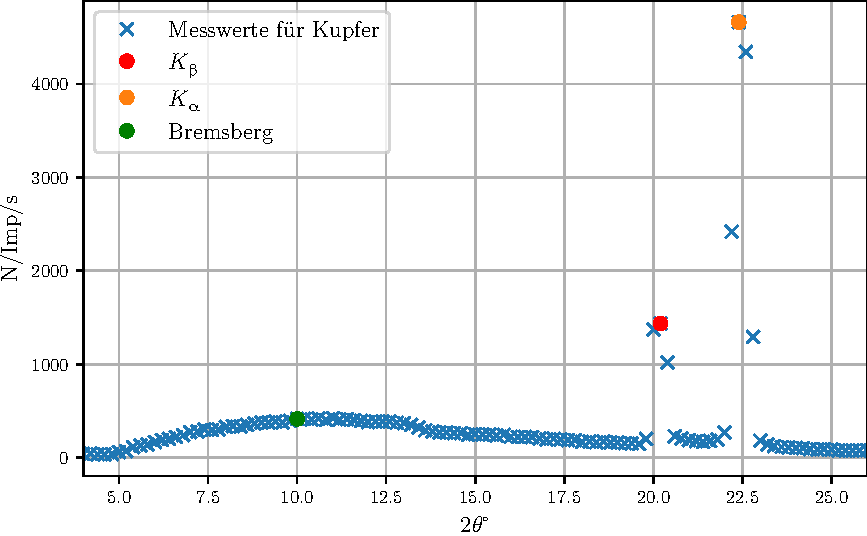
\includegraphics{cu.pdf}
  \caption{Emissionsspektrum der Cu-Röntgenröhre.}
  \label{fig:cu}
\end{figure}
In \autoref{fig:cu} wird das Emissionspektrum dargestellt. Die $K_{\symup{\alpha}}$-, $K_{\symup{\beta}}$-Linie und
der Bremsberg werden aus den Messwerten durch Ablesen bestimmt. Die Halbwertsbreite (FWHM) bestimmt sich aus dem
Detailspektrum wieder durch Ablesen, so dass die Angabe eines statistischen Fehlers nicht nötig ist.
Die $K_{\symup{\alpha}}$-Linie befindet sich bei $2\theta=22,4^{\circ}$ und 
$N = 4662\,\frac{\symup{Imp}}{\unit{\second}}$. Die $K_{\symup{\beta}}$-Linie befindet sich bei 
$2\theta=20,2^{\circ}$ und $N = 1437\,\frac{\symup{Imp}}{\unit{\second}}$. Die Halbwertsbreiten bestimmen sich zu
\begin{align*}
  \theta_{\symup{FWHM, \alpha}} &= 0,55^{\circ} \; \symup{und} \\
  \theta_{\symup{FWHM, \beta}} &= 0,55^{\circ}. 
\end{align*}
Daraus und der Bragg-Bedingung aus \autoref{eqn:bragg} lassen sich nun die minimalen Wellenlängen bzw.
die maximale Energie $E = \frac{hc}{\lambda}$ bestimmen zu
\begin{align*}
  E_{K,\alpha}           &= 3,095\,\unit{\kilo\eV},\\
  E_{K, \beta}           &= 4,924\,\unit{\kilo\eV},\\
  \Delta E_{FWHM,\alpha} &= 1,849\,\unit{\kilo\eV} \; \symup{und}\\
  \Delta E_{FWHM,\beta}  &= 0,219\,\unit{\kilo\eV}.
\end{align*}
Das Auflösungsvermögen bestimmt sich durch
\begin{align*}
  A = \frac{E_{\symup{K}}}{\Delta E_{\symup{FWHM}}}.
\end{align*}
Für die $K_{\symup{\alpha}}$-Linie und $K_{\symup{\beta}}$-Linie bestimmt sich das Auflösungsvermögen zu
\begin{align*}
  A_{\symup{K}_{\alpha}}  &=  1,67 \; \symup{und}\\
  A_{\symup{K}_{\beta}}   &= 22,50.
\end{align*}
Die Absorptionskoeffizienten bestimmen sich durch \autoref{eqn:Ekabs}, \autoref{eqn:EKa} und
\autoref{eqn:EKb} zu
\begin{align*}
  \sigma_{\symup{1}} &= ,\\
  \sigma_{\symup{2}} &= ,\\
  \sigma_{\symup{3}} &= .
\end{align*}